\documentclass[12pt,a4paper, margin=3in]{article}
\usepackage[utf8]{inputenc}
\usepackage[margin=.75in]{geometry}
\usepackage{amsmath}
\usepackage{tikz}
\usepackage{physics}
\usepackage{diffcoeff}

\setlength{\parindent}{0em}
\setlength{\parskip}{2em}

\begin{document}

\subsection*{1) Derive the far-field radiation pattern for a combination of a dipole antenna placed at the focus of a parabolic dish. Assume that the dipole illuminates the whole aperture of the dish uniformly.
}

\large 

\subsection*{2) Why can we practically not have a uniformly illuminated aperture like the previous case? What is an optimal solution in the practical scenario to maximize the telescope's performance?
}

\large A uniform illumination means a sharp fall in the aperture distribution graph close to the edge of the parabola, just like the case of the uniform line aperture. Because of these sharp features in the aperture distribution, its fourier transform (which gives us the far-field radiation pattern) will have large values for large $\theta$, meaning that the dish will have large side-lobes. Large side-lobes are undesirable as they add noise from ground, man-made sources etc. This is why, uniform apertures illumination with a sharp profile is avoided. 

It is observed that the more the aperture distribution is made to fall gradually from the center of the dish to the edge, the more the side-lobes get smaller. This gradual fall-off is called 'taper' and real aperture distributions are designed to have some taper. However, the width of the main-lobe/primary beam (by which we are actually observing) increases with higher taper. A very wide main-lobe is undesirable since the gain in the primary beam decreases for wider main-lobe. In addition, the resolution of the telescope is high for thinner main-lobe. 

Hence there are 2 opposing effects: high taper reduces side lobes but also reduces gain of the primary beam. In practical scenario, an optimal solution involves having the taper to an extent which keeps the gain and side-lobes around acceptable levels. For low-noise receivers a compromise is usually reached when the taper is between −12 and −15 dB at the edge \footnote{Source - 'An Introduction to Radio Astronomy'- Bernard F. Burke, Francis Graham-Smith, Peter N. Wilkinson (2019)}. 

\newpage 

\subsection*{3) Given the impulse response of a linear device like a filter or amplifier, what is the output of the device for an input signal?
}

\large The impulse response of a linear time-invariant (LTI) system $h(t)$ is the output of the system for a very short impulse input (mathematically, a delta function input for continuous signals). Any general input $x(t)$ can be intuitively chopped into very thin intervals which resemble a series of such scaled and time-shifted impulse functions. The input then can be interpreted as a sum of these impulse functions. The system being linear would act on the these individual impulses separately with their respective scaling being preserved. Hence the output would look like a series of scaled and time-shifted impulse responses and adding them all up would give the output signal $y(t). 

Adding all these scaled and shifted impulse responses means that at $t= t_0,  y(t_0) $ will be the sum of all impulse function values with each value scaled by the values of $x(t)$, like a weighted sum. The way the weighted sum comes out is that the value $h(t_0 - \tau)$ is weighted by $x(\tau)$. So $y(t = t_0)$ is equal to $h(t_0 - \tau)\,x(\tau)$ summed over $\tau$. In integral form this becomes - \begin{equation}y(t = t_0) = \int_{-\infty} ^{\infty} h(t_0 - \tau) \cdot{x(\tau)} \,d\tau \end{equation} which is nothing but the convolution of $x(t)$ with $h(t)$.  
Therefore for any general input $x(t)$, the output of a linear system is given by the convolution of $x(t)$ with the impulse response of the system, $h(t)$.

\newpage

\large \textit{Meeting on 9th May}

\subsection*{1) Define and express the SNR in terms of the signal properties and explain how a reduction in the noise (through integration for ex) enables us to detect fainter sources.}

\large Consider 2 scenarios. One, where the telescope is not looking at the astronomical source and the other where it is. In the former the signal that comes out of the integrator comprises of all the noise power (and its fluctuations) from various sources; and in the other case, its a sum of noise power and the power from the astronomical source (plus fluctuations). The output of the integrator is a DC signal with its values fluctuating around a mean value which is nothing but the power in the input signal. Let the mean power in the two cases be $P_1$ and $P_2$ respectively. The crucial quantity here is how big are the fluctuations from these mean power values. Let $\sigma$ be the average value of these fluctuations or the standard deviation of the noise distribution. The figure below illustrates the situation - 
\vspace{15mm}

\begin{figure}[htp]
    \centering
    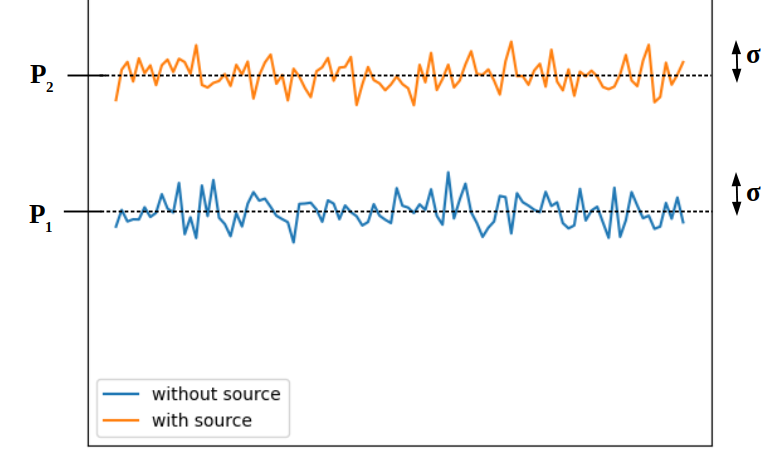
\includegraphics[width=18cm]{image}
\end{figure}

\vspace{15}

The power from the source itself would then be equal to $P_2 - P_1$. This is the 'signal' part in SNR. 'Noise' is directly quantified by $\sigma$, so the 'signal-to-noise ratio' (SNR) would be equal to - \begin{equation}SNR = \frac{P_2 - P_1}{\sigma} \end{equation}

While looking at the sky suppose we get a signal with power $P_2$ such that $P_1 < P_2 < P_1 + \sigma$. In this situation we cant say if $P_2$ corresponds to a real signal, because there is a high probability that those readings are from noise. Only when $P_2$ is greater than multiples of $\sigma$ can we say with some good probability that there is a real astronomical object. Now if we reduce $\sigma$ (by integration for example), the minimum value of $P_2$ for which we can have confidence gets closer and closer to $P_1$ which is the ultimate limit to how sensitive our telescope can be. Thus we can detect sources with lesser and lesser power (till the limit $P_1$) by reducing $\sigma$.

\end{document}

